\section{NP-Completeness}

\vspace{\parskip}

\begin{definition}[NP-complete] \index{NP-complete}
    A language $A$ is \textit{\textbf{NP-complete}} if it is in $\NP$ and every language $B \in \NP$ is polynomial time reducible to $A$. 
\end{definition}

Let $A$ be any NP-complete problem, then $\p = \NP$ if and only if $A \in \p$.

If $A$ is NP-complete, then assuming $\p \neq \NP$ (we don't know if this is true), $A$ is not solvable in time $O(n^k)$ for any $k$.

\section{The Cook-Levin Theorem}

\vspace{\parskip}

\begin{theorem}[Cook and Levin 1971]
    SAT and 3SAT are NP-complete.
\end{theorem}

SAT is the \textit{\textbf{Boolean satisfiability problem}} of propositional formulas.

Boolean variables: $x,y,z,\ldots$ taking values of \const{true} and \const{false} (represented by 1 and 0, respectively).

Boolean operations: AND ($\vee$), OR ($\wedge$), NOT (top bar or $\neg$)

Boolean formula: expressions involving Boolean variables and operations.

A Boolean formula is satisfiable if some assignment of 0s and 1s to its variable makes the formula evaluate to 1.

The satisfiability problem is to test whether a Boolean formula is satisfiable. More formally, consider the language
$$
\SAT = \{ \encoding{\phi} \mid \text{$\phi$ is a satisfiable Boolean formula}\}
$$

Literal: a Boolean variable and its negation.

CNF formula: conjunctive normal form, and of ors. Each group of literals or'ed together is called a clause.

3CNF formula: each clause has 3 literals.

\section{Proof of the Cook-Levin Theorem}

\textit{Proof idea}.

First, we show that $\SAT \in \NP$: there is a polynomial time verifier that checks that a certificate is a satisfying assignment. Alternatively, we can construct an NTM that guesses the satisfying assignments.

Next, we need to show that $\SAT$ is NP-hard, that is, every language in $\NP$ is polynomial time reducible to $\SAT$.

For all $A \in \NP$, show that $A \leq_p \SAT$. Such polynomial time reduction takes a string $w$ and maps it to a formula such $\phi$ such that $w \in A \iff \phi \in \SAT$.

Since $A \in \NP$, there is a constant $k$ and NTM $N$ with running time $n^k$ such that $A = \lang(N)$. $\phi$ will simulate the machine $N$ on $w$ where $A = \lang(N)$.

A tableau for $N$ on $w$ is an $n^k \times (n^k + 3)$ tbale, whose rows are
$$
\# C_0 \#,\,\# C_1 \#,\, \# C_2 \#,\, \ldots,\, \# C_{n^k} \#
$$
where each $C_i$ is a configuration with $n^k$ tape symbols and $C_i$ yields $C_{i+1}$ under $N$'s transition function for all $i \in \{1,\ldots,n^{k-1}\}$.

$N$ accepts $w$ $\iff$ there is an accepting tableau for $N$ on $w$.

A tableau is accepting if and only if $C_i$ is an accepting configuration. We want to construct the formula $\phi$ that will describe all logical constraints tha any accepting tableau for $N$ on $w$ must satisfy.

So,
$$
\text{$\phi$ is satisfiable} \iff \text{there is an accepting tableau for $N$ on $w$} \iff \text{$N$ accepts $w$} 
$$

Let $C = Q \cup \Gamma \cup \{\#\}$ be the alphabet of the tableau (i.e. all characters tha can appear in the tableau).

\begin{itemize}
    \item each entry of the tableau is a cell
    \item cell[$i,j$] denotes the value of the cell at row $i$ and column $j$ 
    \item for every $i,j$ such that $1 \leq i \leq n^k$ and $1 \leq j \leq n^k + 3$ and every $s \in C$, there is a variable $x_{i,j,s}$. $x_{i,j,s}$ is a variable of $\phi$
\end{itemize}

Hence, the total number of variables is $n^k(n^k + 3)|C| \in O(n^{2k})$.

$x_{i,j,s} = 1$ corresponds to cell[$i,j$] = $s$.

We will now design $\phi$ such that any satisfying assignment for $\phi$ corresponds to an accepting tableau for $N$ on $w$.

Formula $\phi$ will be the AND of four CNF formulas
$$
\phi = \phi_{cell} \land \phi_{start} \land \phi_{accept} \land \phi_{move}
$$
where

$\phi_{cell}$: for all $i,j$, exactly one $s \in C$ has $x_{i,j,s} = 1$.
$$
\phi_{cell} = \bigvee_{\substack{1 \leq i \leq n^k \\ 1 \leq j \leq n^k+3}} \left[ \left( \bigwedge_{s \in C} x_{i,j,s} \right) \land \left( \bigvee_{\substack{s,t \in C \\ s \neq t}} \left( \overline{x_{i,j,s}} \lor \overline{x_{i,j,t}} \right)  \right)  \right] 
$$

$\bigwedge_{s \in C} x_{i,j,s}$ enforces that at least one variable is set to 1; $\bigvee_{\substack{s,t \in C \\ s \neq t}} \left( \overline{x_{i,j,s}} \lor \overline{x_{i,j,t}} \right)$ enforces that at most one variable is set to 1.

$\phi_{start}$: the first row of the tableau is the start configuration of $N$ on $w$

$$
\phi_{start} = x_{1,1,\#} \land x_{1,2,q_0} \land x_{1,3,w_1} \land \ldots \land x_{1,n^k+2,\sqcup} \land x_{1,n^k+3, \#}
$$

$\phi_{accept}$: an accepting configuration is last row of the tableau

$$
\phi_{accept} = \bigvee_{\substack{1 \leq i \leq n^k \\ 1 \leq j \leq n^k + 3}} x_{i,j,q_{accept}}
$$

$\phi_{move}$: the tableau is legal, i.e. every row is a configuration that legally follows from the previous configuration

This formula will check that every $2 \times 3$ ``windows'' of cells is legal, i.e. it obeys transition function.

\begin{figure}[htbp]
    \centering
    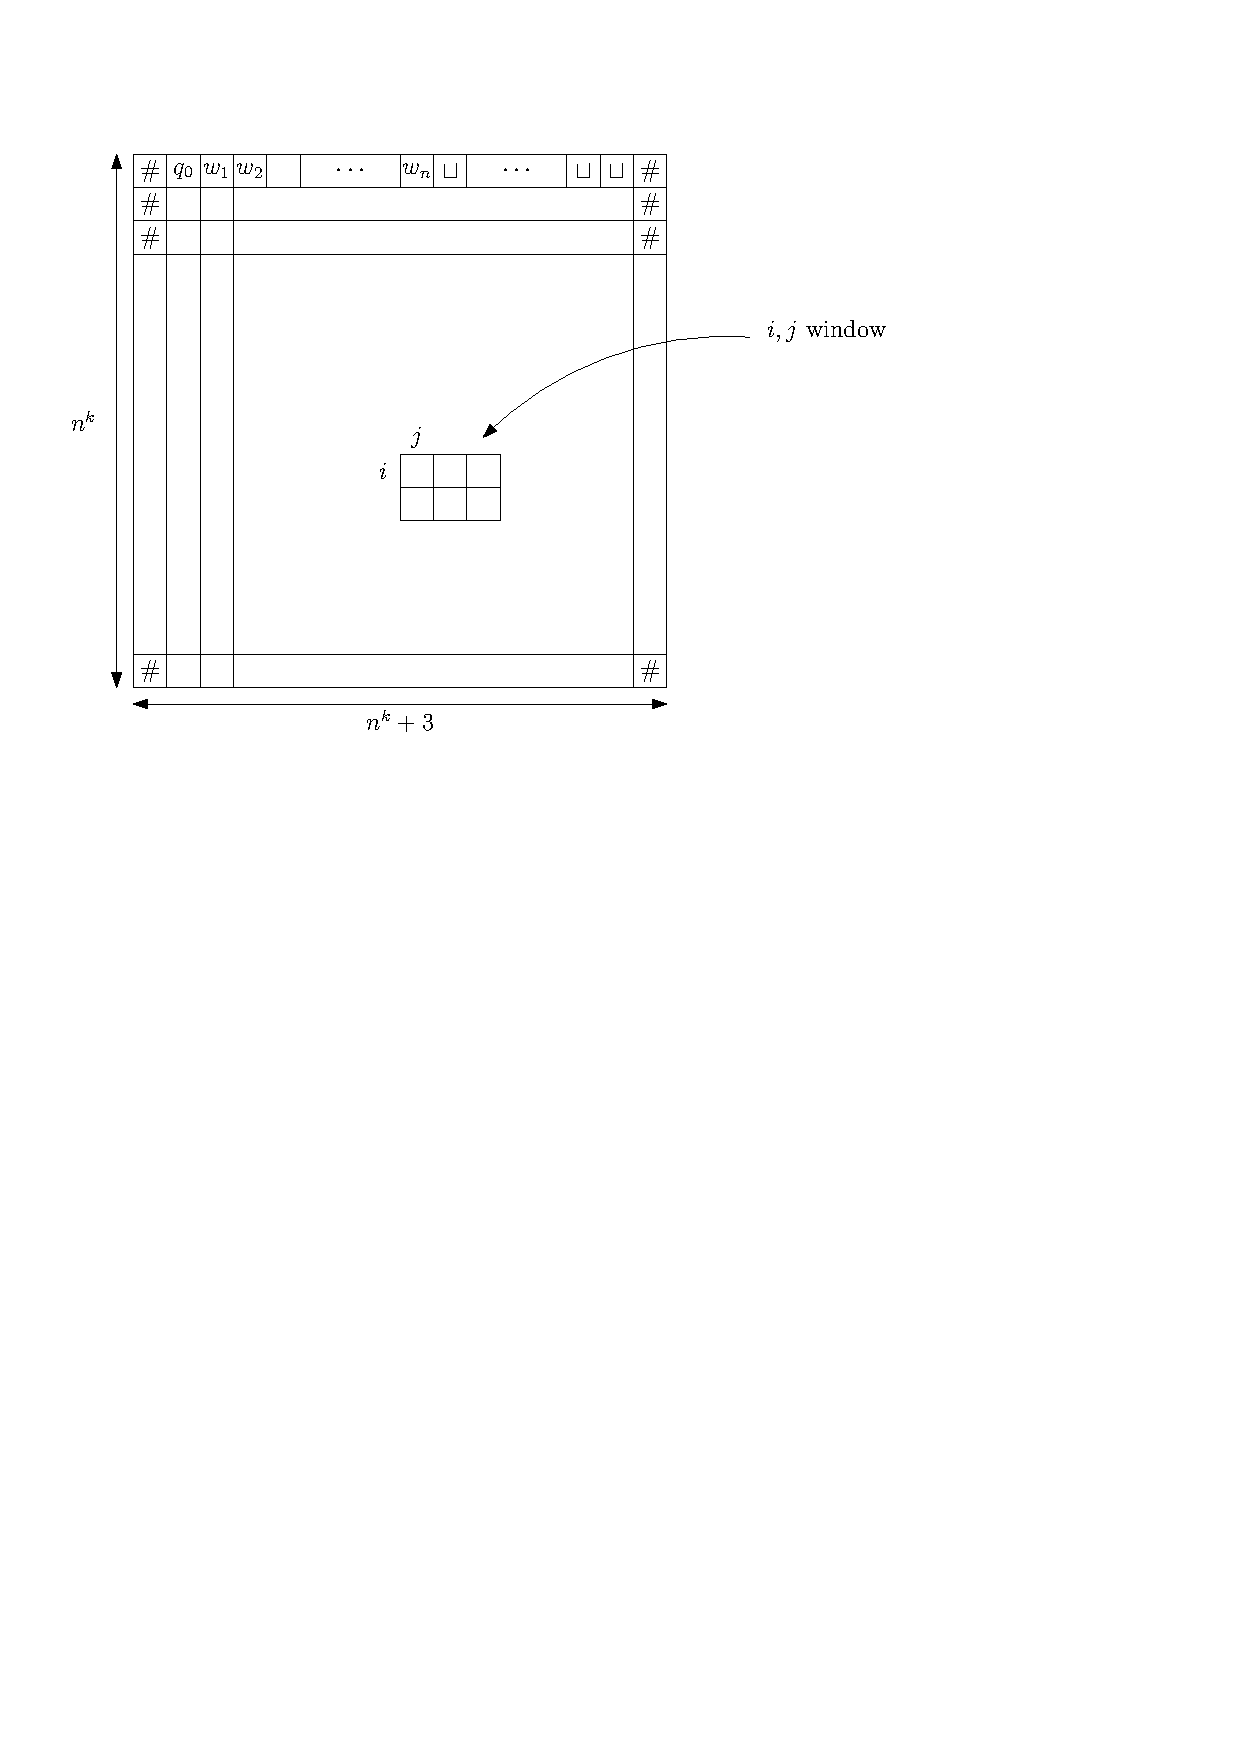
\includegraphics[width=0.7\linewidth]{tableau.pdf}
    \caption{A tableau.}
    \label{fig:cook-levin-tableau}
\end{figure}

Informally,
$$
\phi_{move} = \bigwedge_{\substack{1 \leq i \leq n^k - 1 \\ 1 \leq j \leq n^k + 1}} \left( \text{the $(i,j)$ window is legal} \right) 
$$
We express ``$(i,j)$ window is legal'' using the formula
$$
\bigvee_{\substack{(a_1,a_2,\ldots,a_6) \\ \text{is a legal window}}} \left( x_{i,j,a_1} \land x_{i,j+1,a_2} \land x_{i,j+2,a_3} \land x_{i+1,j,a_4} \land x_{i+1,j+1,a_5} \land x_{i+1,j+2,a_6} \right) 
$$
which is equivalent to
$$
\bigwedge_{\substack{(a_1,\ldots,a_6) \\ \text{isn't a legal window}}} \left( \overline{x_{i,j,a_1}} \lor \overline{x_{i,j+1,a_2}} \lor \overline{x_{i,j+2,a_3}} \lor \overline{x_{i+1,j,a_4}} \lor \overline{x_{i+1,j+1,a_5}} \lor \overline{x_{i+1,j+2,a_6}} \right) 
$$

\begin{figure}[htbp]
    \centering
    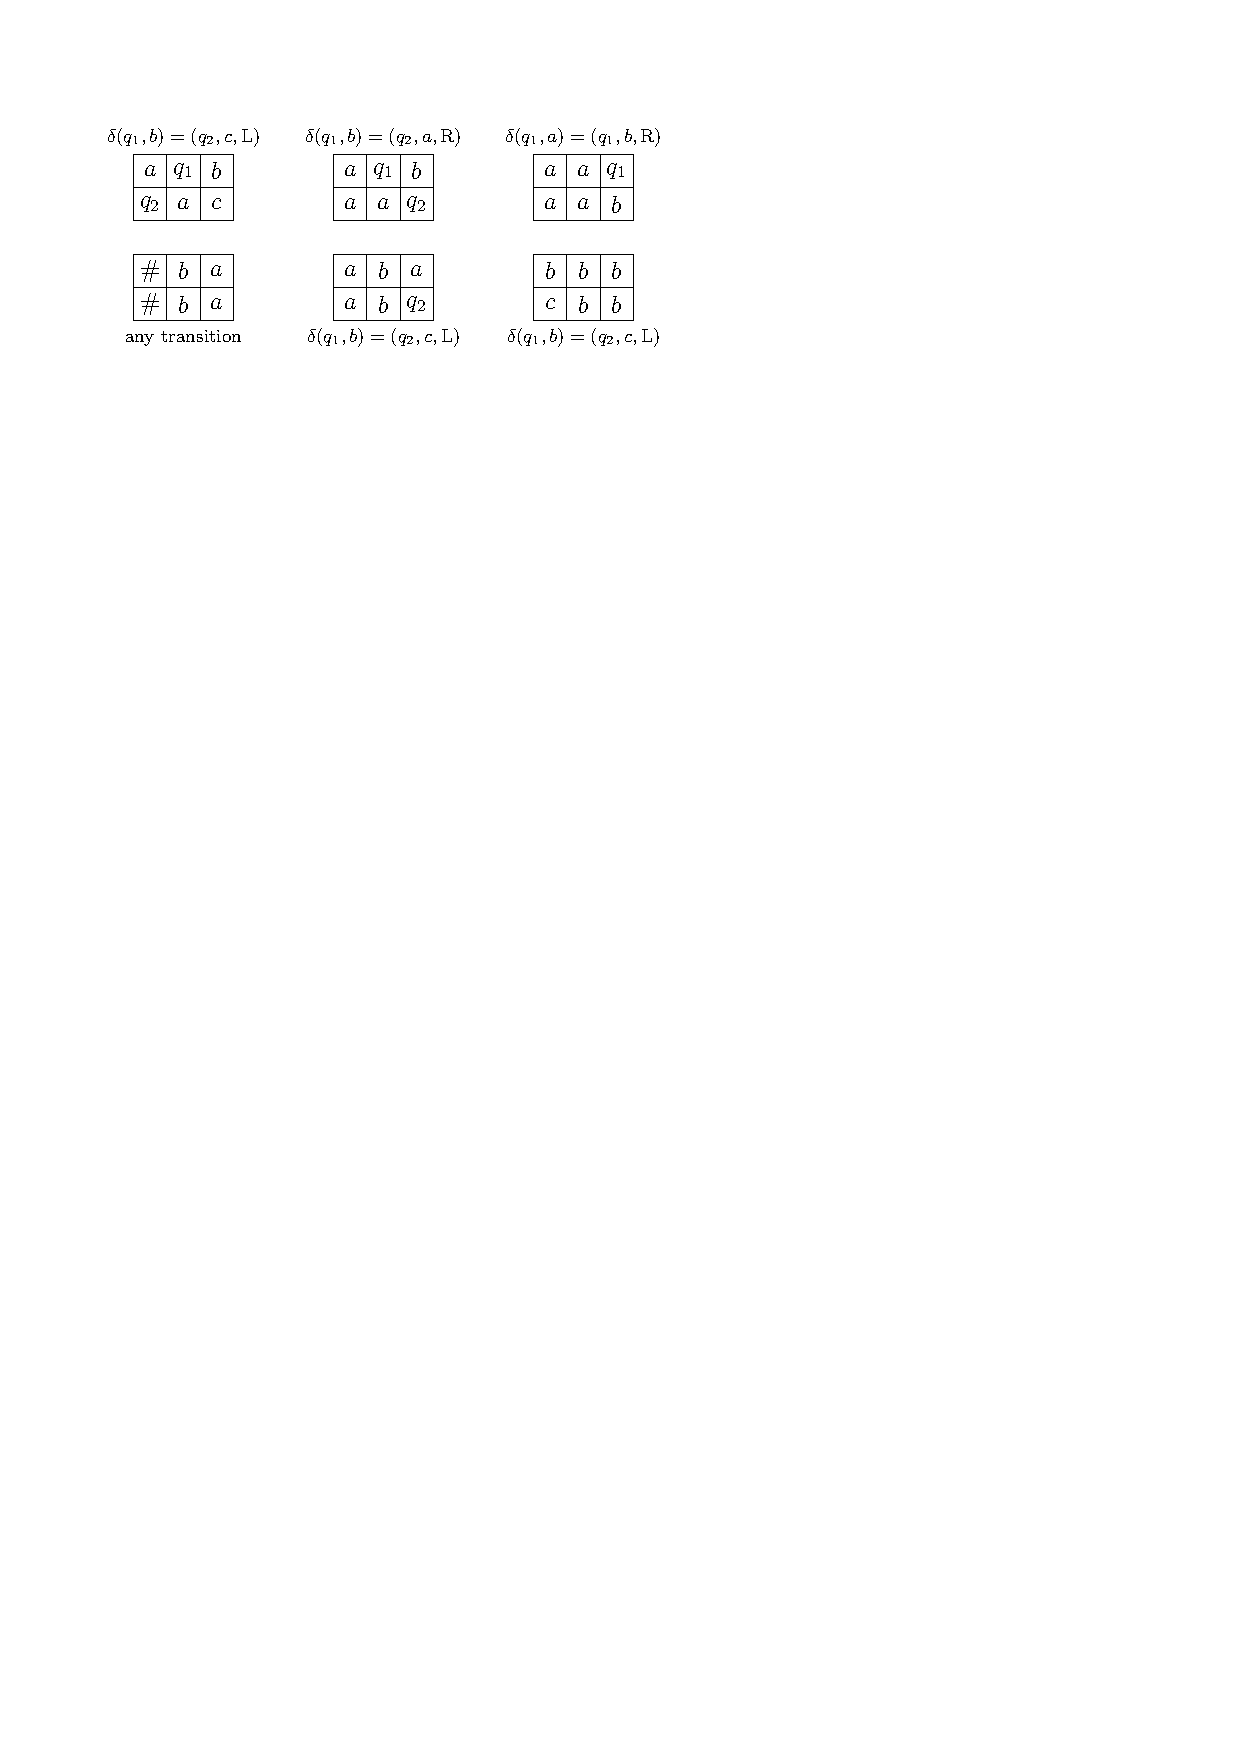
\includegraphics[width=0.6\linewidth]{legal-windows.pdf}
    \caption{Some legal windows under the transition function $\delta(q_1,b) = (q_2,c,\mathrm{L})$, $\delta(q_1,b) = (q_2,a,\mathrm{R})$, and $\delta(q_1,a) = (q_1,b,\mathrm{R})$.  }
    \label{fig:cook-levin-legal-windows}
\end{figure}

\begin{lemma}
    If the top row of the tableau is the start configuration and every window in the tableau is legal, each row of the tableau is a configuration that legally follows the preceding one. In other words, if some configuration does not follow from the previous one, we are guaranteed to detect the violation in some window.
\end{lemma}

\begin{proof}
    See Sipser Claim 7.41.
\end{proof}

Thus $A \leq_p \SAT$ so $\SAT$ is NP-complete.

\section{3SAT}

Everything is already in AND of ORs (CNF), we need to make this ORs small (3CNF). Let's start with a short example of a 4CNF with one clause.
$$
(a_1 \lor a_2 \lor a_3 \lor a_4) \iff (a_1 \lor a_2 \lor z_1) \land (\neg z_1 \lor a_3 \lor a_4)
$$
Every assignment that satisfies the formula on the LHS satisfies the formula on the RHS, and vice versa.

In general, for each clause in the original formula,
$$
(a_1 \lor a_2 \lor a_3 \lor \cdots \lor a_t)
$$
we can replace it with
$$
(a_1 \lor a_2 \lor z_1) \land (\neg z_1 \lor a_3 \lor z_2) \land (\neg z_2 \lor a_4 \lor z_3) \land (\neg z_3 \lor \cdots) \land \cdots \land (\neg z_{t-3} \lor a_{t-1} \lor a_{t})
$$
with $t-2$ clauses.